\documentclass[10pt, compress]{beamer}

\usetheme{m}

\usepackage{booktabs}
\usepackage[scale=2]{ccicons}
\usepackage{minted}

\usemintedstyle{trac}

\title{IR : Article Presentation}
\subtitle{Self-Stabilizing Resource Discovery Algorithm\\\textit{Seda Davtyan, Kishori M. Konwar, Alexander A. Shvartsman}}
\date{\today}
\author{Alexandre Honorat}
\institute{University of Bordeaux Master RSM, supervised by Colette Johnen}

\begin{document}

\maketitle

\section{Introduction}

%%

\begin{frame}{Article topic}

\begin{block}{Resource Discovery Problem (RDP)}
Each resource wants to know all other available resources in the same network.
\end{block}

\begin{block}{Self-Stabilizing Problem [Ref2]}
\alert{Closure} and \alert{convergence}: fault-tolerant.
\end{block}

\begin{exampleblock}{Peer-to-peer networks}
A virtual resource network is built at software level for example in \textsf{Gnutella} [Ref7, Ref15].
\end{exampleblock}

\end{frame}

%%

\begin{frame}{RDP formalism}

\begin{block}{Synchronous model}
\begin{itemize}
\item global clock and synchronized rounds
\item each message sent in a round is received before its end
\end{itemize}
\end{block}

\begin{block}{Knowledge graph [Ref6]}
Directed graph $\mathnormal{G(V,E)}$, initialy weakly connected, \alert{finally complete}.  
\begin{itemize}
\item node = resource
\item edge = knowledge about another resource
\end{itemize}
\end{block}

\begin{block}{Complexity}
\begin{itemize}
\item complexity in time = number of rounds
\item complexity in message = number of messages
\item $\mathnormal{D} =$ graph diameter and $\mathnormal{n = |V|}$.
\end{itemize}
\end{block}

\end{frame}

%%

\begin{frame}{Related Work}

\begin{table}
\caption{Time and message complexity of some algorithms solving RDP in synchronous networks.}
\label{tab:tc}
\begin{center}
\begin{tabular}{||c||c|c||}
\hline
Algorithm & Time & Message \\
\hline
\hline
[Ref9] (lower bounds) & $\mathnormal{\Omega(log \, D)}$ & $\mathnormal{\Omega(n)}$\\
\hline
[Ref6] (randomized) & $\mathnormal{O(log^2 \, n)}$ & $\mathnormal{O(n \, log^2 \, n)}$\\
\hline
[Ref12] (deterministic) & $\mathnormal{O(log \, n)}$ & $\mathnormal{O(n \, log \, n)}$\\
\hline
[Ref13] (randomized) & $\mathnormal{O(log \, n)}$ & $\mathnormal{O(n \, log \, n)}$\\
\hline
Presented algorithm & $\mathnormal{O(D)}$ & $\mathnormal{O(n \cdot D)}$\\
\hline
\end{tabular}
\end{center}
\end{table}

Question: $\mathnormal{D \ll log \, n}$ ?

\end{frame}

%%

\section{Algorithm}

%%

\begin{frame}{Specific formalism}

\begin{block}{Knowledge graph}
A node knows only another one at the beginning.
\end{block}

\begin{block}{Global clock}
$\mathnormal{t}$ is the round duration, $ \mathnormal{t}$ is large enough to ensure that all messages are received before the end of the round. Actually $\mathnormal{t \ll RTT}.$
\end{block}

\begin{block}{Timed Input/Output Automata [Ref8]}
\begin{itemize}
\item \emph{discrete transitions}: evolve immediately %includes send/receive, perturb*, join* or restrart
\item \emph{trajectories}: evolve with the clock%main instructions or reset
\end{itemize}
\end{block}

\end{frame}

%%

\begin{frame}{Overview}

\begin{block}{Variables}
\begin{itemize}
\item $\mathnormal{R}$ the set of nodes from which we received a message
\item $\mathnormal{parent}$ the lowest neighbour id known
\item $\mathnormal{pro\_parent}$ the lowest neighbor parent id known 
\item $\mathnormal{Children}$ the set of nodes self-declared as our children
\item $\mathnormal{Nbrs}$ nodes considering us $\mathnormal{i}$ as their initial neighbor $\mathnormal{j}$ (including itself, in fact $\mathnormal{Nbrs}$ is reset to $\mathnormal{\{i, j\}}$ at each iteration begin)
%\item $\mathnormal{Dest}$ message addressees
\end{itemize}
\end{block}

\begin{block}{Message content}
Nodes can multicast messages always containing its own identifier, its parent identifier, its initial neighbor and its children set.
\end{block}

\end{frame}

%%

\begin{frame}{Working}

\begin{block}{Goal}
All nodes have the same parent (lowest id node), and they consider children of this "root" as the entire network know.
\end{block}

\begin{block}{Iterations}
Two phases (one phase at each round):
\begin{enumerate}
\item{\alert{gossip}: sets $\mathnormal{parent}$ as the minimum id in $\mathnormal{R \cup \{i, j\}}$, sets $\mathnormal{pro\_parent}$, then sends messages to $\mathnormal{parent \cup pro\_parent \cup  Nbrs \cup Children}$ and finally $\mathnormal{Children} \leftarrow \emptyset$\\
\textit{or} \alert{reset}: if $\mathnormal{parent}$ does not appear in $\mathnormal{R}$}
\item{\alert{confirm}: sets $\mathnormal{Children}$ and $\mathnormal{Nbrs}$ to children and neighbors discovered in \alert{gossip} phase, then send message to $\mathnormal{R \cup Nbrs}$}
\end{enumerate}
\end{block}

\end{frame}

%%

\begin{frame}{Self-stabilization: closure}

\begin{block}{Resource Discovery Invariant}
We have reached a legitimate state when:
\begin{enumerate}
\item For every node $\mathnormal{v \in V}$, $\mathnormal{v}$ is active and $\mathnormal{parent_v = min\{u\,:\, u \in V\}}$.
\item There exists a node $\mathnormal{v_0 \in V}$ such that $\mathnormal{v_0 = min\{u\,:\, u \in V\}}$ and $\mathnormal{Children_{v_0} = V}$, while for every other node $\mathnormal{w \neq v_0}$, with $\mathnormal{w \in V}$, we have $\mathnormal{Children_w = \emptyset}$.
\end{enumerate}
\end{block}

\begin{block}{Failure formalism}
All variables, messages and even program counter can be corrupted. $\mathnormal{t}$, $\mathnormal{\{i, j\}}$ and the clock cannot be corrupted.
\end{block}

\end{frame}

%%

\begin{frame}{Self-stabilization: convergence}

\begin{block}{Adding a node -- case 1: \qquad
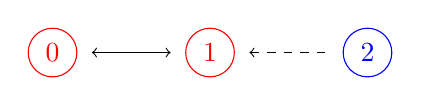
\begin{tikzpicture}
\node[draw, circle, red] at (0,0) {$0$};
\draw[<->] (0.5,0) -- (1.5,0);
\node[draw, circle, red] at (2,0) {$1$};
\draw[<-,dashed] (2.5,0) -- (3.5,0);
\node[draw, circle, blue] at (4,0) {$2$};
\end{tikzpicture}
}
\begin{enumerate}
\item (gossip) 2 contacts 1, 1 puts it in $Nbrs_1$
\item (confirm) 1 contacts 2, 2 puts 1's parent (i. e. 0) in $pro\_parent_2$
\item (g.) 2 contacts 0, but 2's parent is still 1
\item (c.) 0 responds to 2
\item (g.) 0 and 2 have a parent/children relation
\item (c.) $K_{0,1,2}$ is set properly with $\{0, 1, 2\}$
\end{enumerate}
\end{block}

\begin{block}{Adding a node -- case 2: \qquad 
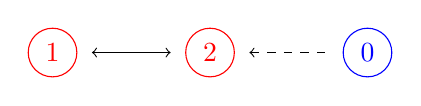
\begin{tikzpicture}
\node[draw, circle, red] at (0,0) {$1$};
\draw[<->] (0.5,0) -- (1.5,0);
\node[draw, circle, red] at (2,0) {$2$};
\draw[<-,dashed] (2.5,0) -- (3.5,0);
\node[draw, circle, blue] at (4,0) {$0$};
\end{tikzpicture}
}
It takes 4 complete iterations (8 rounds) to reach a legitimate state.
\end{block}

\begin{block}{Complexity}
$\mathnormal{O(D)}$ in time and $\mathnormal{O(n \cdot D)}$ in messages
\end{block}
\end{frame}

%%

\section{Conclusion}

%%

\begin{frame}{Pros and cons}
    \begin{exampleblock}{Pros}
    \begin{itemize}
    \item fault-tolerant
    \item \textit{probably} fast
    \end{itemize}
    \end{exampleblock}
    \begin{alertblock}{Cons}
    \begin{itemize}
    \item $\mathnormal{t}$ must be known in advance
    \item must check if initial graph is weakly connected
    \item if the root fails, algorithm restart from begining
    \item amount of data exchanged
    \end{itemize}
    \end{alertblock}
\end{frame}

%%

\plain{}{Questions}

\end{document}
